\documentclass[10pt]{article}

% Official TMLR review style from the JMLR organization. Only two non-executable
% contact comments were removed; do not change formatting statements or enable
% the accepted/preprint option during review.
\usepackage{tmlr}
\usepackage{amsmath}
\usepackage{booktabs}
\usepackage{graphicx}
\usepackage{hyperref}
\usepackage{url}

\graphicspath{{figures/}}

\title{Uncertainty-Aware Belief Supervision under Persistent Hidden Thermal
Dynamics: Evidence from Two Robot-Control Tasks}

% The review style suppresses this field, but the source is also kept anonymous
% so that accidental style changes cannot reveal author information.
\author{Anonymous Authors}

% Camera-ready placeholders required by the official style.
\def\month{MM}
\def\year{YYYY}
\def\openreview{\url{https://openreview.net/forum?id=XXXX}}

\begin{document}

\maketitle

\begin{abstract}
Robot-control benchmarks commonly reset the environment between tasks, hiding
failure modes caused by physical state that accumulates across those resets.
We study fixed low-level controllers in two MuJoCo manipulation tasks where
task state resets but an unobserved, action-driven thermal state persists and
changes later actuator dynamics. An explicit belief supervisor uses a noisy
temperature signal and an uncertainty margin to choose between high- and
low-power control. Under prespecified sensor and cooling shifts, a fresh Pusher
factorial showed that a physics-only uncertainty margin improved mean
risk-sensitive lifetime utility by $+0.965$ reward per task (95\% bootstrap CI
$[0.733,1.196]$), but its maximum trip rate was 2.15\%; the corresponding full
hybrid supervisor had a smaller margin effect ($+0.736$, $[0.524,0.950]$) and a
1.3\% maximum trip rate. On Reacher, the inherited physics-only margin retained
a positive mean effect ($+0.721$, $[0.474,0.978]$) but reached 2.3\%, whereas
the secondary hybrid supervisor reached 1.4\%. A separately frozen development
procedure selected a more conservative physics-only margin; on 100 new Reacher
lifetimes it passed the 2\% tolerance (1.6\%) with a positive mean effect
($+0.692$, $[0.434,0.962]$). The inherited margin also passed on that second
sample (1.9\%), and the calibrated setting had no detectable mean-utility
advantage over it. Only 52 of 100 calibrated lifetime effects were positive.
Thus, uncertainty margins improve expected risk-sensitive utility in this
benchmark, while point trip-rate gates near their boundary depend on policy
composition and evaluation sample. The results establish neither calibration
superiority nor a transferable safety guarantee and are limited to a shared
phenomenological thermal model in simulation.
\end{abstract}

\section{Introduction}
\label{sec:introduction}

Many robot-learning evaluations divide interaction into short tasks and reset
the simulator after each one. This convention is useful for optimization and
comparison, but it can erase internal physical state---such as temperature or
wear---that would survive an ordinary task boundary. Removing embodiment resets
entirely creates its own exploration and learning problem
\citep{farrahi2025continuing}. We study a complementary selective-reset
setting: the arm, object, and goal reset, while a hidden actuator-health state
persists and changes the dynamics faced by later tasks.

Thermal-aware robot learning is not new. Recent quadruped work incorporates
motor-temperature models into reinforcement-learning policies and validates
thermal management on hardware \citep{qian2026thermal,wan2026residual}.
Damage-aware manipulation benchmarks also accumulate thermal and mechanical
health signals across interaction \citep{balaji2026oopsieverse}. Our question
is narrower. We deliberately use a phenomenological thermal law to isolate
what happens when health is hidden, action-driven, persistent across task
resets, and causally changes subsequent actuator dynamics. This controlled
setting is intended to expose a deployment issue, not to predict the
temperature of a physical motor.

The deployed controller has two layers. A fixed low-level policy performs the
manipulation task, while a supervisor chooses between high- and low-power modes
using a belief about the hidden thermal state. The supervisor can enlarge its
belief by an uncertainty margin before making that choice. Such modular
uncertainty-aware filtering has strong precedent, including belief-space and
latent safety filters with substantially stronger guarantees than those studied
here \citep{vahs2024risk,seo2025latent,kwon2026adaptive}. We therefore do not
claim a new safety-filter architecture. Instead, we ask whether a fixed margin
improves lifetime utility under deployment shifts, whether that numerical
margin transfers between robot-control tasks, and what a target-specific
calibration stage actually recovers.

We answer these questions in Pusher and Reacher under matched selective-reset
semantics and a shared thermal law. Each independent evaluation unit is a
20-task lifetime. Sensor-noise, cooling, physical-shock, and combined shifts
are evaluated using paired fresh lifetimes. The experimental sequence keeps
the inherited cross-task test separate from a later, development-only
calibration and its disjoint fresh test set.

The results provide three main findings. First, a fresh Pusher factorial
experiment attributes the robust benefit primarily to the uncertainty margin:
without the learned residual, the margin improves target-shift mean utility by
$+0.965$ reward per task (95\% bootstrap CI $[0.733,1.196]$). Second, the same
margin retains a positive mean effect on Reacher ($+0.721$,
$[0.474,0.978]$) but reaches a 2.3\% maximum trip rate and therefore fails the
prespecified 2.0\% tolerance. Third, a separately frozen calibration using only
Reacher development lifetimes selects a more conservative margin; on 100 new
lifetimes it reaches 1.6\% while preserving a positive mean effect ($+0.692$,
$[0.434,0.962]$). Its mean utility is not detectably different from the
inherited setting. Calibration is therefore credited with tolerance recovery,
not reward superiority.

These are mean risk-sensitive utility results, not universal dominance. Only
52 of 100 calibrated Reacher lifetime effects are positive, and the exact sign
test is not significant. Pusher reward decomposition further shows that fewer
thermal trips compensate for lower immediate task return, so the conclusion
depends on trips carrying moderate or high cost. Together, the evidence
supports a practical and testable workflow---calibrate the uncertainty margin
on target-task development lifetimes, freeze it, and evaluate it once---while
leaving hardware validity, formal safety, and general algorithmic superiority
open.

\section{Related work}
\label{sec:related}

\paragraph{Persistent state and reset semantics.}
Continuing reinforcement learning studies interaction without ordinary episode
or embodiment resets \citep{farrahi2025continuing}. Damage-aware manipulation
benchmarks accumulate health from several physical channels
\citep{balaji2026oopsieverse}. Our selective-reset diagnostic instead restores
the task configuration while retaining only a hidden health state that feeds
back into subsequent dynamics.

\paragraph{Thermal-aware robot control.}
Thermal models, temperature-conditioned policies, and residual thermal control
have been demonstrated in simulation and on quadruped hardware
\citep{qian2026thermal,wan2026residual}. Our model is less physically detailed
and is not calibrated to hardware. It is used to study partial observability,
uncertainty margins, policy composition, and development-only margin selection
under controlled shifts.

\paragraph{Belief and uncertainty-aware supervision.}
Prior work constructs risk-aware control directly in belief space and develops
uncertainty-aware filters for hidden or out-of-distribution dynamics
\citep{vahs2024risk,seo2025latent,kwon2026adaptive}. Those works establish the
architectural and theoretical precedents. Our contribution is empirical:
fresh-lifetime mechanism attribution, explicit separation of physics-only and
hybrid outcomes, and a separately frozen calibration test whose necessity and
superiority are not assumed.

% Before submission, expand this section from the bounded depth-two audit in
% docs/LITERATURE_AUDIT_2026-08-31.md and refresh every closest-work comparison.

\section{Selective-reset problem setting}
\label{sec:problem}

An evaluation lifetime contains 20 manipulation tasks. At each task boundary,
the task configuration is reset while the latent thermal state is retained.
The thermal state changes as a function of selected actions, influences later
actuator efficiency, and is observed by the deployed supervisor only through a
noisy sensor. This produces a partially observed control problem in which a
conventional task reset does not restore the complete physical state.

The reported objective is risk-sensitive lifetime utility: task return and a
small high-power throughput term are balanced against a thermal-trip penalty.
The independent statistical unit is the complete lifetime, never an individual
task. The same phenomenological thermal law is used in both MuJoCo tasks. It is
a controlled experimental mechanism rather than a motor model in physical
units.

% TODO: migrate the exact transition, observation, actuator-efficiency, trip,
% and utility equations from the frozen protocols, preserving notation and
% parameter values verbatim.

\section{Belief supervisor and comparators}
\label{sec:method}

A fixed low-level controller supplies task actions. Above it, a supervisor
selects a high- or low-power mode from an explicit physics belief about the
hidden thermal state. The uncertainty-aware variant adds a multiple $z$ of its
estimated uncertainty before applying a threshold. The Pusher transfer setting
uses $z=1.5$; the separately calibrated Reacher setting uses cutoff 0.06 and
$z=2.0$.

The experiments also include an optional learned residual on the physics
belief, a privileged current-state threshold comparator, and a monolithic
RecurrentPPO baseline. The privileged comparator is diagnostic and is not a
planning oracle. The recurrent result is evidence only about the tested
architecture, development seeds, training budget, and selection procedure.

% TODO: add pseudocode and the exact observation sets available to each policy.
% Keep analysis-only health variables separate from deployment observations.

\section{Evaluation protocol}
\label{sec:evaluation}

The evidential sequence has five stages: Pusher development and confirmation;
a fresh Pusher residual-by-uncertainty factorial; an inherited-margin Reacher
confirmation; post-confirmatory Reacher calibration on development lifetimes;
and one calibrated evaluation on a disjoint set of fresh Reacher lifetimes.
The original Reacher tolerance failure remains unchanged and is not replaced by
the later calibrated result.

The principal comparisons use 100 paired independent lifetimes and aggregate
within lifetime over the prespecified target deployment shifts. We report mean
paired effects, seed-bootstrap 95\% confidence intervals, paired sign-flip
tests, positive-lifetime counts, exact sign tests, and the maximum
condition-level trip rate. A frozen 2.0\% trip-rate tolerance evaluates the
deployed treatment. Raw reward levels are not pooled across Pusher and Reacher
because the task scales differ.

% TODO: add the complete condition table, seed-role table, hashes, test tails,
% resampling counts, and multiplicity handling from the frozen protocols.

\section{Results}
\label{sec:results}

\subsection{Pusher: uncertainty, not the residual, is the robust component}

The fresh $2\times2$ factorial uses 100 independent lifetimes. At matched
$z=1.5$, the residual effect is $+0.103$ reward per task with a 95\% bootstrap
CI of $[-0.004,0.215]$. By contrast, the uncertainty-margin effect is $+0.965$
without the residual ($[0.733,1.196]$) and $+0.736$ with it
($[0.524,0.950]$). The residual-attribution gate does not pass; the main
mechanistic conclusion concerns uncertainty-aware trip avoidance. Importantly,
the physics-only $z=1.5$ treatment reaches a 2.15\% maximum trip rate and thus
misses the 2.0\% point tolerance. The complete hybrid $z=1.5$ treatment reaches
1.3\% and passes it. The $+0.965$ effect and the 1.3\% rate therefore describe
different contrasts and must not be combined into one policy claim.

\begin{figure}[t]
  \centering
  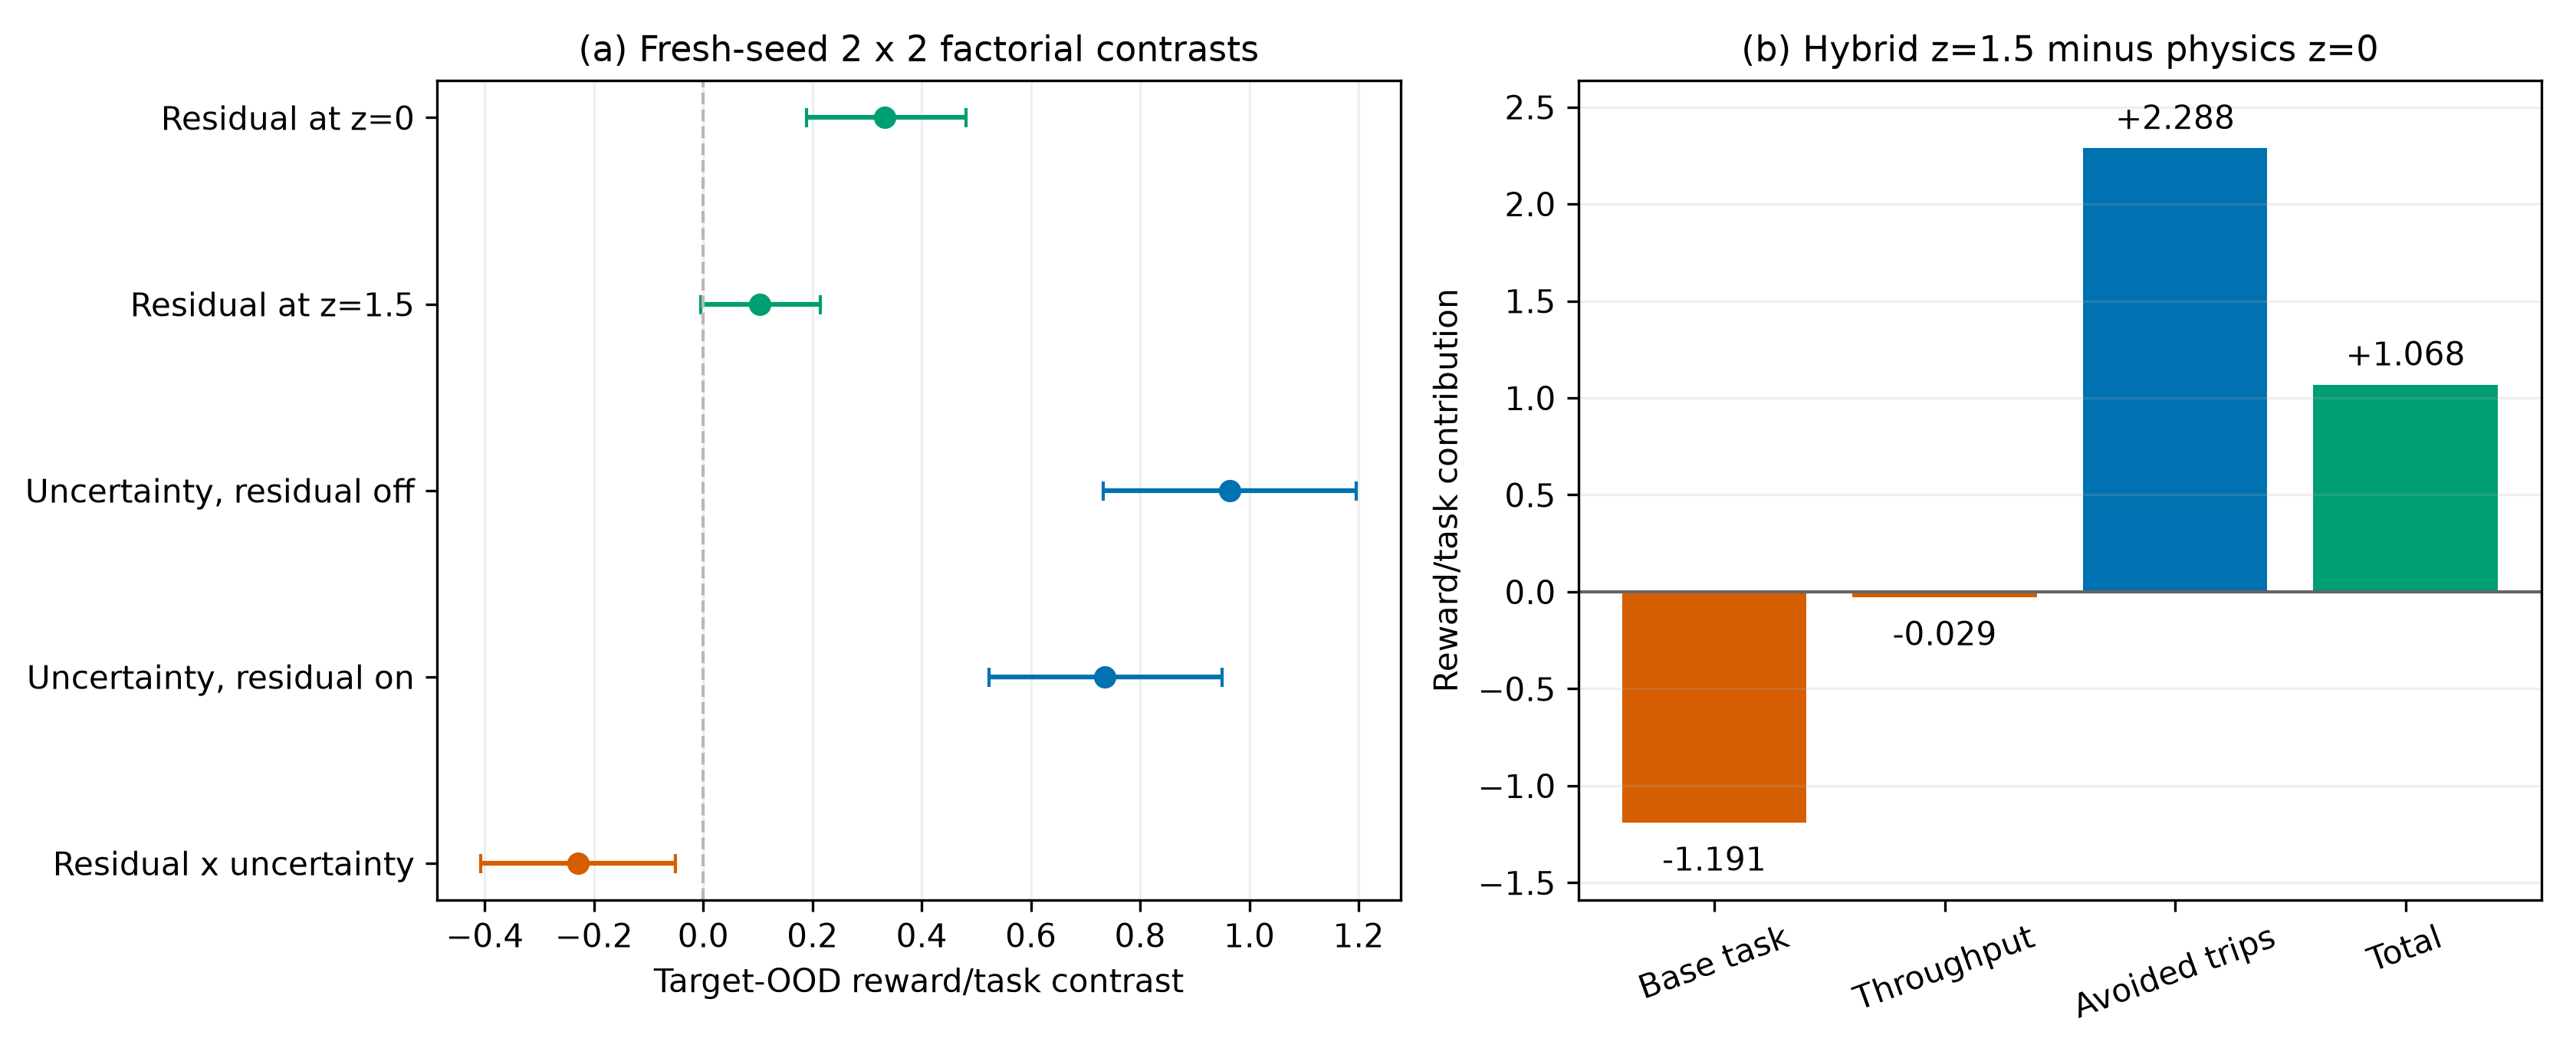
\includegraphics[width=\linewidth]{figure_pusher_factorial.png}
  \caption{Fresh-lifetime Pusher factorial contrasts. The uncertainty margin
  has the larger and more stable effect; the residual contribution at the
  deployed margin is not independently established.}
  \label{fig:pusher-factorial}
\end{figure}

\subsection{Reacher: positive mean effects near the tolerance boundary}

The inherited $z=1.5$ margin improves mean target-shift utility over $z=0$ by
$+0.721$ reward per task ($[0.474,0.978]$). Its maximum trip rate is 2.3\%,
however, so the frozen 2.0\% gate fails. The magnitude-sensitive mean result and
the failed empirical tolerance are both retained. A secondary full-hybrid
comparison improves utility by $+0.797$ ($[0.546,1.059]$) relative to physics
$z=0$ and reaches a 1.4\% maximum trip rate.

\subsection{Development-only calibration yields a passing designated policy}

A prespecified grid evaluated only on Reacher development lifetimes selects
cutoff 0.06 and $z=2.0$ using a buffered 1.5\% rule. On 100 new lifetimes, the
selected policy improves mean utility over $z=0$ by $+0.692$
($[0.434,0.962]$) and reaches a 1.6\% maximum trip rate. Its mean effect relative
to inherited $z=1.5$ is $-0.008$ ($[-0.121,0.108]$), so calibration places the
selected policy on the passing side of the point rule without a detectable
expected-utility loss rather than improving mean reward. On this
same fresh extension sample, however, the inherited $z=1.5$ policy also passes
at 1.9\%. The experiment therefore demonstrates a feasible development-only
selection procedure, but not that calibration was necessary, superior, or the
cause of passing the fresh gate.

\begin{figure}[t]
  \centering
  
\includegraphics[width=\linewidth]{figure_reacher_replication_summary.png}
  \caption{Reacher inherited-margin confirmation and separately frozen
  calibrated-margin extension. The inherited failure remains the authoritative
  zero-shot transfer outcome.}
  \label{fig:reacher-summary}
\end{figure}

Only 52 of 100 calibrated lifetime effects are positive, and the exact sign
test is not significant ($p=0.764$). The result supports a paired mean
expected-utility claim, not improvement in a majority of lifetimes.

\begin{table*}[t]
  \centering
  \small
  \caption{Principal and prespecified secondary results. The maximum trip rate
  is the treatment maximum across the five evaluation conditions. A value
  above 2.0\% fails the frozen point rule. All five paired mean contrasts have
  two-sided sign-flip $p\leq3\times10^{-6}$.}
  \label{tab:principal-results}
  \resizebox{\textwidth}{!}{%
  \begin{tabular}{lllrrrr}
    \toprule
    Task & Contrast & Mean effect & 95\% CI & Positive & Exact sign $p$ & Max trip \\
    \midrule
    Pusher & physics $z=1.5$ vs. $z=0$ & 0.965 & [0.733, 1.196] & 77/100 & $5.5\times10^{-8}$ & 2.15\% \\
    Pusher & hybrid $z=1.5$ vs. $z=0$ & 0.736 & [0.524, 0.950] & 72/100 & $1.26\times10^{-5}$ & 1.30\% \\
    Reacher & physics $z=1.5$ vs. $z=0$ & 0.721 & [0.474, 0.978] & 54/100 & 0.484 & 2.30\% \\
    Reacher & hybrid $z=1.5$ vs. physics $z=0$ & 0.797 & [0.546, 1.059] & 62/100 & 0.021 & 1.40\% \\
    Reacher & calibrated physics $z=2$ vs. $z=0$ & 0.692 & [0.434, 0.962] & 52/100 & 0.764 & 1.60\% \\
    \bottomrule
  \end{tabular}}
\end{table*}

\section{Discussion and limitations}
\label{sec:discussion}

The combined evidence supports a deployment workflow within this benchmark:
retain an explicit belief over persistent physical state, select the
conservatism margin on target-task development lifetimes using a buffered
tolerance, freeze the choice, and evaluate it once on fresh lifetimes. A margin
can improve average utility on a new task yet still miss a prespecified
trip-rate tolerance, so positive transfer of reward is not sufficient evidence
for transferring a numerical operating threshold.

The utility improvement is not free. In Pusher, avoided trip cost outweighs a
decrease in immediate base-task return, and fixed-trajectory reweighting places
the mean break-even trip penalty near 40 under the original throughput bonus.
This accounting sensitivity is not policy retraining and does not establish a
benefit when trips carry little cost.

Both tasks use MuJoCo and share one phenomenological thermal law. The study has
no physical-unit calibration, hardware telemetry, formal safety proof, or
probability-calibrated OOD guarantee. It tests one selected recurrent baseline
rather than exhausting recurrent, meta-RL, system-identification, or online
adaptation methods. These boundaries prevent the result from supporting a
general thermal-management or universal algorithm-ranking claim.

\section{Broader impact}

Persistent-health benchmarks may help reveal controllers that trade short-term
performance for lower accumulated risk. The same abstractions could also be
misused to overstate safety when simulated health signals are poorly calibrated
or when an aggregate trip tolerance hides rare severe outcomes. We mitigate
this risk by preserving failed gates, reporting distributional cautions,
avoiding physical-validity claims, and releasing the exact simulated protocol
needed to inspect the result. The computational cost and environmental impact
of training and evaluation will be reported in the final manuscript.

\section{Conclusion}
\label{sec:conclusion}

Uncertainty-aware belief supervision improved mean risk-sensitive lifetime
utility in two controlled manipulation tasks. Physics-only $z=1.5$ policies
missed the 2\% point trip-rate rule in the designated Pusher and Reacher tests,
whereas the corresponding complete hybrid policies passed; the residual's own
incremental contribution was not established. A target-development procedure
selected a more conservative Reacher physics-only policy that passed on a new
sample, but the inherited policy also passed there and neither calibration
superiority nor necessity was demonstrated. The result is a two-task
simulation study about uncertainty-aware control under persistent hidden
dynamics, not a hardware, transferable-threshold, or formal safety guarantee.
More generally, persistent-state studies should preserve the lifetime as the
evaluation unit and should not treat an expected-utility gain, a point-rate
gate, and evidence for calibration as interchangeable conclusions.


\bibliography{references}
\bibliographystyle{tmlr}

\appendix
\section{Protocol and artifact details}
\label{app:protocol}

The final appendix will contain the complete environment equations, parameter
tables, seed-role manifests, protocol and checkpoint hashes, condition-level
results, calibration frontier, recurrent training details, reward sensitivity,
and artifact-reproduction commands. All primary evidence required to interpret
the central claim remains in the paper body because appendix review is
discretionary.


\end{document}
